% Chapter 22: System Identification
% IEEE-formatted LaTeX chapter for Control Systems Textbook
% Self-contained chapter - can be \input{} into main document

\chapter{System Identification}
\label{ch:system_identification}


%=============================================================================
\section{Historical Motivation: Learning Models from Data}
\label{sec:sysid_history}
%=============================================================================

The challenge of building accurate mathematical models has confronted engineers and scientists for centuries. While physics provides elegant equations governing idealized systems, real-world systems exhibit complexities---nonlinearities, distributed parameters, unknown friction, parasitic dynamics---that make first-principles modeling extraordinarily difficult. System identification offers an alternative: rather than deriving models from physical laws, we learn them directly from observed input-output behavior.

\subsection{Gauss and the Birth of Least Squares (1809)}
\label{subsec:gauss}

\begin{historicalbox}[Carl Friedrich Gauss and the Method of Least Squares]
Carl Friedrich Gauss (1777--1855), often called the ``Prince of Mathematicians,'' developed the method of least squares as a young man of 24. When the asteroid Ceres was discovered in 1801, Gauss used his new technique to compute its orbit from just 41 days of observations---a feat that astonished the astronomical community when Ceres was successfully relocated in December 1801, exactly where Gauss predicted. Though Adrien-Marie Legendre published the method first in 1805, Gauss had used it privately since 1795. Gauss published his full theory in 1809 in \textit{Theoria Motus Corporum Coelestium}, where he also introduced the normal distribution (``Gaussian'' distribution) as the natural error model justifying least squares. His work established the foundation for all modern statistical estimation, from signal processing to machine learning. Gauss's insight that squared errors lead to mathematically tractable and statistically optimal estimates remains one of the most influential ideas in applied mathematics.
\end{historicalbox}

The mathematical foundations of system identification trace to Carl Friedrich Gauss and his work on celestial mechanics. In 1801, the Italian astronomer Giuseppe Piazzi discovered Ceres, the first asteroid, observing it for only 41 days before it disappeared behind the Sun. The astronomical community faced a critical challenge: with such limited observations, could Ceres's orbit be predicted well enough to relocate it months later when it emerged from the Sun's glare?

\subsubsection{The Orbit Prediction Problem}

The orbit of a celestial body is described by six parameters: semi-major axis, eccentricity, inclination, longitude of ascending node, argument of perihelion, and true anomaly. However, observational measurements contain errors from atmospheric distortion, instrument imprecision, and human factors. Given $n$ noisy observations where $n > 6$, how should one estimate the six orbital parameters?

The challenge is \textit{overdetermined}: more equations than unknowns. Different subsets of observations yield different parameter estimates. Which estimate is ``best''?

\subsubsection{Gauss's Method of Least Squares}

Gauss proposed a principle that would become the cornerstone of statistical estimation: choose the parameters that minimize the sum of squared errors between predicted and observed positions. If $y_i$ denotes the $i$-th observed position and $\hat{y}_i(\boldsymbol{\theta})$ the position predicted by model parameters $\boldsymbol{\theta}$, the optimal estimate is:
\begin{equation}
\hat{\boldsymbol{\theta}} = \arg\min_{\boldsymbol{\theta}} \sum_{i=1}^{n} \left( y_i - \hat{y}_i(\boldsymbol{\theta}) \right)^2
\label{eq:gauss_ls}
\end{equation}

Using this method, the 24-year-old Gauss computed Ceres's orbit with such accuracy that astronomer Franz Xaver von Zach relocated the asteroid on December 31, 1801---within half a degree of Gauss's prediction. This triumph established least squares as the fundamental tool for fitting models to data.

\subsubsection{Why Squared Errors?}

Gauss justified the squared error criterion through his theory of errors. Under the assumption that measurement errors are normally distributed (the ``Gaussian'' distribution he characterized), the least squares estimate is also the \textit{maximum likelihood} estimate---the parameter values most likely to have produced the observed data. This provided a principled statistical foundation for what might otherwise seem an arbitrary choice.

The squared error criterion also offers practical advantages. The squared function is smooth everywhere, enabling gradient-based optimization through differentiability. For linear-in-parameters models, the objective function is convex, guaranteeing a unique global minimum. Linear least squares admits a closed-form solution via the normal equations, providing analytical tractability. Furthermore, under Gaussian noise assumptions, least squares achieves statistical optimality as the Best Linear Unbiased Estimator (BLUE).

\subsection{From Astronomy to Engineering}
\label{subsec:engineering_history}

Throughout the 19th and early 20th centuries, least squares remained primarily a tool of astronomers and surveyors. Engineers building control systems relied on first-principles models derived from Newton's laws, thermodynamics, and electrical circuit theory. However, several developments gradually pushed engineers toward data-driven approaches.

\subsubsection{The Complexity Barrier}

As engineered systems grew more sophisticated, first-principles modeling became increasingly burdensome. Aircraft flutter analysis required predicting the complex interaction between aerodynamic forces and structural vibration, demanding models of extraordinary complexity; finite element methods could approximate structural dynamics, but coupling with unsteady aerodynamics introduced uncertainties that pure analysis could not resolve. In process control, chemical plants involve thousands of interacting variables---temperatures, pressures, flow rates, concentrations---with nonlinear kinetics and transport phenomena, making complete mechanistic models impractical for online control. Electromechanical systems presented their own challenges, as friction, backlash, magnetic saturation, and thermal effects created discrepancies between idealized models and actual behavior.

\subsubsection{The Data Revolution}

Simultaneously, the ability to collect experimental data improved dramatically. Electronic sensors---including strain gauges, thermocouples, and later solid-state sensors---enabled precise measurement of physical quantities. Data acquisition systems with analog-to-digital converters and digital storage made it feasible to record thousands of data points. Digital computers provided the computational power to process large datasets and perform the matrix operations required for least squares.

The economics shifted: collecting data became cheaper than developing first-principles models.

\subsection{Lennart Ljung and the Modern Framework (1970s--1980s)}
\label{subsec:ljung}

The modern theory of system identification crystallized through the work of Lennart Ljung at Link\"{o}ping University in Sweden. His 1987 textbook \textit{System Identification: Theory for the User} synthesized decades of research into a coherent framework that remains the foundation of the field.

\subsubsection{Ljung's Contributions}

Ljung's framework addressed several critical questions. First, model structure selection: what class of models should we consider, given that too simple a structure cannot capture system dynamics while too complex a structure leads to overfitting? Second, input design: what input signals maximize the information content of experimental data? Third, estimation algorithms: how do we efficiently compute optimal parameter estimates, especially for nonlinear model structures? Fourth, model validation: how do we assess whether an identified model is adequate for its intended purpose? Finally, theoretical foundations: under what conditions do parameter estimates converge to true values as data increases?

\subsubsection{The Prediction Error Framework}

Central to Ljung's approach is the \textit{prediction error method}. Given a model parametrized by $\boldsymbol{\theta}$, define the one-step-ahead prediction:
\begin{equation}
\hat{y}(t|\boldsymbol{\theta}) = \text{best prediction of } y(t) \text{ given past data and model } \boldsymbol{\theta}
\end{equation}

The prediction error is:
\begin{equation}
\varepsilon(t, \boldsymbol{\theta}) = y(t) - \hat{y}(t|\boldsymbol{\theta})
\end{equation}

The parameter estimate minimizes a criterion function of these errors:
\begin{equation}
\hat{\boldsymbol{\theta}}_N = \arg\min_{\boldsymbol{\theta}} V_N(\boldsymbol{\theta}) = \arg\min_{\boldsymbol{\theta}} \frac{1}{N} \sum_{t=1}^{N} \ell\left(\varepsilon(t, \boldsymbol{\theta})\right)
\label{eq:pem}
\end{equation}
where $\ell(\cdot)$ is a loss function (typically $\ell(\varepsilon) = \varepsilon^2$ for quadratic loss).

This framework unifies diverse identification methods---least squares, maximum likelihood, instrumental variables---as special cases with different model structures and loss functions.

\subsection{``All Models Are Wrong, Some Are Useful''}
\label{subsec:box}

The statistician George E.P. Box articulated a crucial philosophical principle that underlies all system identification work:

\begin{quote}
``Essentially, all models are wrong, but some are useful.'' --- George E.P. Box, 1976
\end{quote}

This aphorism captures several important truths. No model is perfect: every mathematical model is a simplification of reality, as real systems have infinite degrees of freedom while models have finite parameters. Usefulness is context-dependent, meaning a model adequate for one purpose may be inadequate for another; a first-order approximation might suffice for slow control loops but fail for high-bandwidth applications. The goal is not truth, but utility: we seek models that predict well within their intended domain of application, not models that capture every physical detail. Finally, model validation is essential; since all models are wrong, we must rigorously test whether a particular model is ``wrong enough to matter'' for our application.

\subsection{Aerospace Applications: Flutter Testing}
\label{subsec:flutter}

Aircraft flutter---the potentially catastrophic interaction between aerodynamic forces and structural vibration---provides a compelling application of system identification. Flight testing for flutter requires extracting dynamic characteristics from in-flight data.

\subsubsection{The Flutter Problem}

As aircraft speed increases, aerodynamic forces couple increasingly strongly with structural modes. At a critical speed, this coupling can produce self-excited oscillations of rapidly growing amplitude---flutter. Since flutter can destroy an aircraft within seconds, flight test programs must carefully approach the flutter boundary while ensuring adequate safety margins.

\subsubsection{Ground Vibration Testing}

Before flight, aircraft undergo ground vibration testing (GVT) to identify structural modes. Shakers excite the structure, and accelerometers measure the response. From this input-output data, modal frequencies, damping ratios, and mode shapes are extracted using system identification techniques.

\subsubsection{Flight Flutter Testing}

In flight, atmospheric turbulence or controlled excitation (from stick inputs, oscillating control surfaces, or dedicated excitation systems) provides the input. The challenge is more severe than ground testing due to several factors: atmospheric turbulence excites all modes simultaneously as multiple inputs; airspeed, altitude, and fuel state change during maneuvers, creating varying conditions; safety concerns limit input amplitude near the flutter boundary, constraining excitation levels; and damping trends must be monitored during the test point, imposing real-time requirements.

Modern flutter testing relies on recursive identification algorithms that update model estimates as data arrives, enabling real-time tracking of modal damping as conditions change.

%=============================================================================
\section{Modern Applications}
\label{sec:sysid_applications}
%=============================================================================

System identification has become indispensable across engineering disciplines, enabling applications ranging from adaptive control to digital twin creation.

\subsection{Adaptive Control: Identify Then Control}
\label{subsec:adaptive}

Adaptive control systems adjust their parameters in response to changing plant dynamics or operating conditions. A common architecture is \textit{indirect adaptive control}, which proceeds as follows: first, an online identification algorithm estimates plant parameters from recent input-output data; then, the estimated parameters are used to update controller gains; finally, this process repeats continuously during operation.

This ``identify then control'' paradigm enables systems to maintain performance despite plant variations---wear, fouling, load changes---that would degrade fixed-gain controllers. Applications span multiple domains: autopilots must handle aircraft dynamics that vary with altitude, speed, and configuration; engine control systems must adapt as combustion characteristics change with temperature and fuel quality; and robot manipulators must accommodate payload mass that varies between tasks.

\subsection{Digital Twins from Operational Data}
\label{subsec:digital_twins}

A \textit{digital twin} is a virtual replica of a physical asset that mirrors its behavior in real-time. System identification enables the creation of digital twins from operational data for several purposes. Predictive maintenance benefits from identifying changes in system dynamics that can reveal incipient faults---bearing wear manifests as changing resonance frequencies, while valve degradation appears as changing flow coefficients. Process optimization leverages high-fidelity models to enable simulation-based optimization without risky experimentation on the physical plant. Operator training uses digital twins to provide realistic simulators for training scenarios.

\subsection{Machine Learning for Dynamics}
\label{subsec:ml}

The boundary between system identification and machine learning has become increasingly porous. Neural network dynamics models, including recurrent networks and transformers, can learn complex nonlinear dynamics from data. Gaussian processes provide probabilistic models with uncertainty quantification. Physics-informed learning combines data-driven fitting with physical constraints such as conservation laws and symmetries. Reinforcement learning uses learned dynamics models for model-predictive control.

These methods extend the reach of system identification to systems too complex for traditional linear or low-order nonlinear models.

\subsection{Biomedical System Modeling}
\label{subsec:biomedical}

Biological systems present unique identification challenges---they cannot be opened for inspection, they vary between individuals, and they adapt over time. System identification enables advances across biomedical applications. Pharmacokinetic modeling estimates drug absorption, distribution, metabolism, and excretion rates from blood concentration measurements. Glucose-insulin dynamics identification produces patient-specific models for artificial pancreas control. Cardiovascular modeling characterizes heart pump function and vascular resistance from pressure and flow measurements. Neural system identification infers neural connectivity and dynamics from electrode recordings or imaging data.

%=============================================================================
\section{Mathematical Foundation}
\label{sec:sysid_math}
%=============================================================================

We now develop the mathematical framework for system identification, proceeding from problem formulation through model structures, estimation algorithms, and validation techniques.

\subsection{Problem Formulation}
\label{subsec:problem_setup}

The fundamental system identification problem can be stated as:

\begin{tcolorbox}[colback=blue!5!white,colframe=blue!75!black,title=System Identification Problem,sharp corners]
\textbf{Given:} A sequence of input measurements $\{u(1), u(2), \ldots, u(N)\}$, a sequence of output measurements $\{y(1), y(2), \ldots, y(N)\}$, and a model structure $\mathcal{M}$ with parameters $\boldsymbol{\theta}$.

\textbf{Find:} The parameter values $\hat{\boldsymbol{\theta}}$ that best explain the observed data according to some criterion.
\end{tcolorbox}

The key choices in this formulation involve three fundamental decisions. The model structure determines what class of models we consider: linear versus nonlinear, continuous versus discrete, parametric versus nonparametric. The optimality criterion defines what ``best'' means---whether least squares, maximum likelihood, or prediction accuracy. Experimental design addresses what inputs should be applied to maximize information content.

\subsection{Input Signal Design}
\label{subsec:input_design}

The input signal profoundly affects identification quality. A constant input provides no information about dynamics. An ideal input excites all relevant modes while respecting practical constraints (amplitude limits, safety, operating range).

\subsubsection{Persistence of Excitation}

For parameter convergence, the input must be \textit{persistently exciting} of sufficient order. Informally, an input is persistently exciting of order $n$ if it contains at least $n$ distinct frequency components. A formal definition involves the positive definiteness of certain correlation matrices:
\begin{equation}
\frac{1}{N} \sum_{t=1}^{N} \boldsymbol{\phi}(t) \boldsymbol{\phi}^T(t) > \alpha \mathbf{I}
\end{equation}
for some $\alpha > 0$, where $\boldsymbol{\phi}(t)$ is the regression vector.

\subsubsection{Pseudorandom Binary Sequence (PRBS)}

A PRBS is a deterministic binary signal that approximates white noise over a finite period. It switches between two levels ($+A$ and $-A$) according to a linear feedback shift register:

\begin{figure}[htbp]
\centering
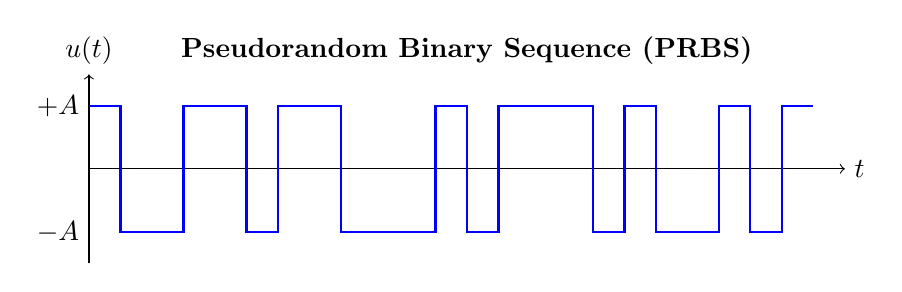
\begin{tikzpicture}[scale=0.8]
    % Time axis
    \draw[->] (0,0) -- (12,0) node[right] {$t$};
    \draw[->] (0,-1.5) -- (0,1.5) node[above] {$u(t)$};

    % PRBS signal
    \draw[thick, blue] (0,1) -- (0.5,1) -- (0.5,-1) -- (1,-1) -- (1,-1) -- (1.5,-1) -- (1.5,1) -- (2,1) -- (2,1) -- (2.5,1) -- (2.5,-1) -- (3,-1) -- (3,1) -- (3.5,1) -- (3.5,1) -- (4,1) -- (4,-1) -- (4.5,-1) -- (4.5,-1) -- (5,-1) -- (5,-1) -- (5.5,-1) -- (5.5,1) -- (6,1) -- (6,-1) -- (6.5,-1) -- (6.5,1) -- (7,1) -- (7,1) -- (7.5,1) -- (7.5,1) -- (8,1) -- (8,-1) -- (8.5,-1) -- (8.5,1) -- (9,1) -- (9,-1) -- (9.5,-1) -- (9.5,-1) -- (10,-1) -- (10,1) -- (10.5,1) -- (10.5,-1) -- (11,-1) -- (11,1) -- (11.5,1);

    % Level labels
    \node[left] at (0,1) {$+A$};
    \node[left] at (0,-1) {$-A$};

    % Title
    \node[above] at (6,1.5) {\textbf{Pseudorandom Binary Sequence (PRBS)}};
\end{tikzpicture}
\caption{A PRBS input signal switches between two levels in a pattern that approximates white noise.}
\label{fig:prbs}
\end{figure}

The PRBS possesses several desirable properties for system identification. Its autocorrelation approximates a delta function, providing broadband excitation with uniform spectral content. The bounded amplitude respects actuator limits. Being deterministic, the signal enables repeatable experiments. The adjustable bandwidth is controlled through the clock frequency, which sets the spectral rolloff.

\subsubsection{Frequency Sweep (Chirp)}

A chirp signal is a sinusoid with time-varying frequency:
\begin{equation}
u(t) = A \sin\left(2\pi f_0 t + \pi \frac{f_1 - f_0}{T} t^2\right)
\label{eq:chirp}
\end{equation}
where frequency sweeps from $f_0$ to $f_1$ over duration $T$.

The chirp is particularly useful for frequency domain identification, exciting each frequency in sequence and enabling spectral analysis at each frequency.

\subsubsection{Step and Pulse Sequences}

Step inputs are simple to implement and intuitive to analyze but concentrate energy at low frequencies. Multiple steps of varying amplitude improve high-frequency content. Pulse sequences (short-duration steps) provide broader excitation.

\subsubsection{Multisine Signals}

A multisine consists of superimposed sinusoids at selected frequencies:
\begin{equation}
u(t) = \sum_{k=1}^{K} A_k \sin(2\pi f_k t + \phi_k)
\end{equation}

By choosing frequencies $f_k$ and phases $\phi_k$, one can target specific frequency bands while controlling the signal's crest factor (ratio of peak to RMS amplitude).

\subsection{Least Squares Estimation}
\label{subsec:least_squares}

Least squares provides the foundation for linear system identification. We develop the method in detail, as it underlies many more sophisticated techniques.

\subsubsection{The Regression Form}

Consider a system whose output depends linearly on known functions of past inputs and outputs:
\begin{equation}
y(t) = \phi_1(t) \theta_1 + \phi_2(t) \theta_2 + \cdots + \phi_n(t) \theta_n + e(t)
\label{eq:regression_scalar}
\end{equation}
where $\phi_i(t)$ are known regressors, $\theta_i$ are unknown parameters, and $e(t)$ is the equation error.

In vector form:
\begin{equation}
y(t) = \boldsymbol{\phi}^T(t) \boldsymbol{\theta} + e(t)
\label{eq:regression_vector}
\end{equation}
where $\boldsymbol{\phi}(t) = [\phi_1(t), \ldots, \phi_n(t)]^T$ and $\boldsymbol{\theta} = [\theta_1, \ldots, \theta_n]^T$.

Collecting $N$ measurements into matrices:
\begin{equation}
\underbrace{\begin{bmatrix} y(1) \\ y(2) \\ \vdots \\ y(N) \end{bmatrix}}_{\mathbf{y}} = \underbrace{\begin{bmatrix} \boldsymbol{\phi}^T(1) \\ \boldsymbol{\phi}^T(2) \\ \vdots \\ \boldsymbol{\phi}^T(N) \end{bmatrix}}_{\boldsymbol{\Phi}} \underbrace{\begin{bmatrix} \theta_1 \\ \theta_2 \\ \vdots \\ \theta_n \end{bmatrix}}_{\boldsymbol{\theta}} + \underbrace{\begin{bmatrix} e(1) \\ e(2) \\ \vdots \\ e(N) \end{bmatrix}}_{\mathbf{e}}
\label{eq:matrix_form}
\end{equation}

Compactly:
\begin{equation}
\mathbf{y} = \boldsymbol{\Phi} \boldsymbol{\theta} + \mathbf{e}
\label{eq:regression_matrix}
\end{equation}

\subsubsection{The Normal Equations}

The least squares estimate minimizes the sum of squared errors:
\begin{equation}
\hat{\boldsymbol{\theta}} = \arg\min_{\boldsymbol{\theta}} J(\boldsymbol{\theta}) = \arg\min_{\boldsymbol{\theta}} \sum_{t=1}^{N} e^2(t) = \arg\min_{\boldsymbol{\theta}} \|\mathbf{y} - \boldsymbol{\Phi}\boldsymbol{\theta}\|^2
\label{eq:ls_criterion}
\end{equation}

Expanding the squared norm:
\begin{equation}
J(\boldsymbol{\theta}) = (\mathbf{y} - \boldsymbol{\Phi}\boldsymbol{\theta})^T (\mathbf{y} - \boldsymbol{\Phi}\boldsymbol{\theta}) = \mathbf{y}^T\mathbf{y} - 2\boldsymbol{\theta}^T\boldsymbol{\Phi}^T\mathbf{y} + \boldsymbol{\theta}^T\boldsymbol{\Phi}^T\boldsymbol{\Phi}\boldsymbol{\theta}
\end{equation}

Taking the gradient and setting to zero:
\begin{equation}
\frac{\partial J}{\partial \boldsymbol{\theta}} = -2\boldsymbol{\Phi}^T\mathbf{y} + 2\boldsymbol{\Phi}^T\boldsymbol{\Phi}\boldsymbol{\theta} = \mathbf{0}
\end{equation}

Solving yields the \textbf{normal equations}:

\begin{tcolorbox}[colback=green!5!white,colframe=green!75!black,title=Least Squares Solution,sharp corners]
\begin{equation}
\hat{\boldsymbol{\theta}} = \left(\boldsymbol{\Phi}^T\boldsymbol{\Phi}\right)^{-1}\boldsymbol{\Phi}^T\mathbf{y}
\label{eq:normal_equations}
\end{equation}

The matrix $\left(\boldsymbol{\Phi}^T\boldsymbol{\Phi}\right)^{-1}\boldsymbol{\Phi}^T$ is the \textit{Moore-Penrose pseudoinverse} of $\boldsymbol{\Phi}$.
\end{tcolorbox}

\subsubsection{Existence and Uniqueness}

The solution (\ref{eq:normal_equations}) exists and is unique if and only if $\boldsymbol{\Phi}^T\boldsymbol{\Phi}$ is invertible. This requires two conditions: first, $N \geq n$, ensuring at least as many measurements as parameters; second, $\text{rank}(\boldsymbol{\Phi}) = n$, ensuring the regressors are linearly independent.

The second condition is equivalent to persistent excitation. If the input is not persistently exciting of order $n$, some parameters are not uniquely identifiable from the data.

\subsubsection{Statistical Properties}

Under the assumption that $e(t)$ is zero-mean white noise with variance $\sigma^2$, the least squares estimate has desirable statistical properties. The estimate is unbiased, meaning $E[\hat{\boldsymbol{\theta}}] = \boldsymbol{\theta}_0$ (the true parameters). It is consistent, with $\hat{\boldsymbol{\theta}} \to \boldsymbol{\theta}_0$ as $N \to \infty$. Furthermore, the estimate achieves minimum variance: among all linear unbiased estimators, least squares has the smallest variance, as established by the Gauss-Markov theorem.

The covariance of the estimate is:
\begin{equation}
\text{Cov}(\hat{\boldsymbol{\theta}}) = \sigma^2 \left(\boldsymbol{\Phi}^T\boldsymbol{\Phi}\right)^{-1}
\label{eq:param_covariance}
\end{equation}

This fundamental result relates estimation uncertainty to noise variance and information content (encoded in $\boldsymbol{\Phi}^T\boldsymbol{\Phi}$).

\subsection{ARX Model Structure}
\label{subsec:arx}

The AutoRegressive with eXogenous input (ARX) model is the simplest and most widely used structure for discrete-time identification.

\subsubsection{Model Definition}

The ARX model relates output $y[k]$ to past outputs, past inputs, and a noise term:
\begin{equation}
y[k] + a_1 y[k-1] + \cdots + a_{n_a} y[k-n_a] = b_1 u[k-1] + \cdots + b_{n_b} u[k-n_b] + e[k]
\label{eq:arx_time}
\end{equation}

Using the backward shift operator $q^{-1}$ (where $q^{-1}y[k] = y[k-1]$):
\begin{equation}
A(q^{-1}) y[k] = B(q^{-1}) u[k] + e[k]
\label{eq:arx_operator}
\end{equation}
where:
\begin{align}
A(q^{-1}) &= 1 + a_1 q^{-1} + a_2 q^{-2} + \cdots + a_{n_a} q^{-n_a} \\
B(q^{-1}) &= b_1 q^{-1} + b_2 q^{-2} + \cdots + b_{n_b} q^{-n_b}
\end{align}

\subsubsection{Transfer Function Form}

The deterministic part of the ARX model corresponds to the transfer function:
\begin{equation}
G(q^{-1}) = \frac{B(q^{-1})}{A(q^{-1})} = \frac{b_1 q^{-1} + b_2 q^{-2} + \cdots + b_{n_b} q^{-n_b}}{1 + a_1 q^{-1} + \cdots + a_{n_a} q^{-n_a}}
\label{eq:arx_tf}
\end{equation}

Converting to $z$-transform notation (where $z = q$):
\begin{equation}
G(z) = \frac{b_1 z^{-1} + \cdots + b_{n_b} z^{-n_b}}{1 + a_1 z^{-1} + \cdots + a_{n_a} z^{-n_a}} = \frac{b_1 z^{n_b-1} + \cdots + b_{n_b}}{z^{n_a} + a_1 z^{n_a-1} + \cdots + a_{n_a}} \cdot z^{n_a - n_b}
\label{eq:arx_z}
\end{equation}

\subsubsection{Regression Form for ARX}

The ARX model (\ref{eq:arx_time}) is linear in the parameters $\{a_1, \ldots, a_{n_a}, b_1, \ldots, b_{n_b}\}$. Rearranging:
\begin{equation}
y[k] = -a_1 y[k-1] - \cdots - a_{n_a} y[k-n_a] + b_1 u[k-1] + \cdots + b_{n_b} u[k-n_b] + e[k]
\end{equation}

Defining:
\begin{align}
\boldsymbol{\phi}[k] &= [-y[k-1], \ldots, -y[k-n_a], u[k-1], \ldots, u[k-n_b]]^T \\
\boldsymbol{\theta} &= [a_1, \ldots, a_{n_a}, b_1, \ldots, b_{n_b}]^T
\end{align}

We obtain the standard regression form:
\begin{equation}
y[k] = \boldsymbol{\phi}^T[k] \boldsymbol{\theta} + e[k]
\end{equation}

The least squares solution (\ref{eq:normal_equations}) directly provides parameter estimates.

\subsubsection{Advantages and Limitations}

The ARX model structure offers several advantages: it reduces to simple linear regression with a closed-form solution, enables efficient computation without iterative optimization, and possesses well-understood statistical properties. However, the structure also has limitations. It assumes a specific noise structure where equation error enters directly. Estimates become biased if the noise is colored (correlated). High model orders may be required to capture complex dynamics adequately.

\subsection{Frequency Domain Identification}
\label{subsec:freq_domain}

An alternative to time-domain parametric identification is to characterize the system's frequency response directly.

\subsubsection{The Frequency Response Function}

For a stable LTI system, the frequency response function (FRF) describes the gain and phase at each frequency:
\begin{equation}
G(j\omega) = |G(j\omega)| e^{j\angle G(j\omega)}
\label{eq:frf}
\end{equation}

The FRF relates sinusoidal inputs to outputs: if $u(t) = A\sin(\omega t)$, then at steady state:
\begin{equation}
y(t) = A|G(j\omega)|\sin(\omega t + \angle G(j\omega))
\label{eq:sinusoidal_ss}
\end{equation}

\subsubsection{Sine-Sweep Identification}

A direct method to measure the FRF proceeds as follows. Apply a sinusoidal input at frequency $\omega_k$ and wait for transients to decay. Measure the output amplitude $Y_k$ and phase $\phi_k$ relative to the input. Compute $|G(j\omega_k)| = Y_k / U_k$ and $\angle G(j\omega_k) = \phi_k$. Repeat this process for frequencies spanning the range of interest.

The result is an \textit{empirical Bode plot}---gain and phase data at discrete frequencies.

\subsubsection{Spectral Analysis}

For broadband inputs (PRBS, random noise), spectral analysis provides FRF estimates:
\begin{equation}
\hat{G}(j\omega) = \frac{S_{yu}(\omega)}{S_{uu}(\omega)}
\label{eq:spectral_frf}
\end{equation}
where $S_{yu}(\omega)$ is the cross-spectral density between output and input, and $S_{uu}(\omega)$ is the input power spectral density.

This approach is computationally efficient using the Fast Fourier Transform (FFT):
\begin{equation}
\hat{G}(j\omega_k) = \frac{Y(\omega_k)}{U(\omega_k)}
\label{eq:fft_frf}
\end{equation}
where $Y(\omega_k)$ and $U(\omega_k)$ are the FFTs of output and input.

\subsubsection{From Frequency Data to Parametric Models}

Once FRF data is available, a parametric model can be fitted:
\begin{equation}
\hat{\boldsymbol{\theta}} = \arg\min_{\boldsymbol{\theta}} \sum_{k=1}^{K} \left| \hat{G}(j\omega_k) - G(j\omega_k; \boldsymbol{\theta}) \right|^2
\label{eq:freq_fitting}
\end{equation}

This frequency-domain fitting can be solved using least squares if the model is linear in parameters, or iterative methods for general rational transfer functions.

\subsection{Model Validation}
\label{subsec:validation}

An identified model must be validated before use. Validation assesses whether the model adequately represents the system for its intended purpose.

\subsubsection{Residual Analysis}

The residuals $\varepsilon(t) = y(t) - \hat{y}(t)$ contain information about model quality. Whiteness is the primary criterion: if the model captures all system dynamics, residuals should be white noise (uncorrelated). Residuals should also demonstrate independence from the input, being uncorrelated with past inputs. Under Gaussian noise assumptions, residuals should exhibit normality, following a normal distribution.

\begin{figure}[htbp]
\centering
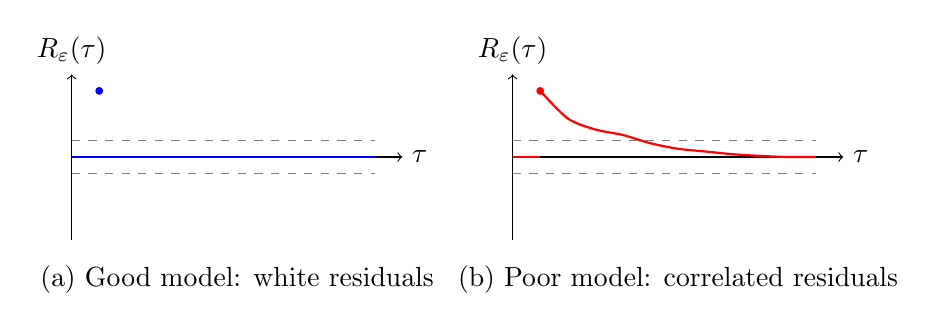
\begin{tikzpicture}[scale=0.7]
    % Good residuals - white noise like
    \begin{scope}
        \draw[->] (0,0) -- (6,0) node[right] {$\tau$};
        \draw[->] (0,-1.5) -- (0,1.5) node[above] {$R_\varepsilon(\tau)$};

        % Autocorrelation of white noise - spike at 0
        \draw[thick, blue] (0,0) -- (0.5,0);
        \draw[thick, blue, fill=blue] (0.5,1.2) circle (0.05);
        \draw[thick, blue] (0.5,0) -- (5.5,0);

        % Confidence bounds
        \draw[dashed, gray] (0,0.3) -- (5.5,0.3);
        \draw[dashed, gray] (0,-0.3) -- (5.5,-0.3);

        \node[below] at (3,-1.8) {(a) Good model: white residuals};
    \end{scope}

    % Bad residuals - correlated
    \begin{scope}[xshift=8cm]
        \draw[->] (0,0) -- (6,0) node[right] {$\tau$};
        \draw[->] (0,-1.5) -- (0,1.5) node[above] {$R_\varepsilon(\tau)$};

        % Autocorrelation showing correlation
        \draw[thick, red] (0,0) -- (0.5,0);
        \draw[thick, red, fill=red] (0.5,1.2) circle (0.05);
        \draw[thick, red] plot[smooth] coordinates {(0.5,1.2) (1,0.7) (1.5,0.5) (2,0.4) (2.5,0.25) (3,0.15) (3.5,0.1) (4,0.05) (4.5,0.02) (5,0) (5.5,0)};

        % Confidence bounds
        \draw[dashed, gray] (0,0.3) -- (5.5,0.3);
        \draw[dashed, gray] (0,-0.3) -- (5.5,-0.3);

        \node[below] at (3,-1.8) {(b) Poor model: correlated residuals};
    \end{scope}
\end{tikzpicture}
\caption{Residual autocorrelation analysis. (a) White residuals indicate the model captures system dynamics. (b) Correlated residuals suggest unmodeled dynamics.}
\label{fig:residual_analysis}
\end{figure}

The autocorrelation function of residuals is:
\begin{equation}
\hat{R}_\varepsilon(\tau) = \frac{1}{N} \sum_{t=1}^{N-\tau} \varepsilon(t)\varepsilon(t+\tau)
\label{eq:residual_acf}
\end{equation}

For a good model, $\hat{R}_\varepsilon(\tau) \approx 0$ for $\tau \neq 0$ (within confidence bounds).

\subsubsection{Cross-Validation}

The gold standard for validation is testing on data not used for estimation. The procedure begins by dividing available data into \textit{estimation} and \textit{validation} sets. The model is identified using only estimation data. The identified model is then simulated with validation input, and the simulated output is compared to the measured validation output.

Common metrics for cross-validation include the fit percentage:
\begin{equation}
\text{FIT} = 100 \times \left(1 - \frac{\|\mathbf{y}_\text{val} - \hat{\mathbf{y}}\|}{\|\mathbf{y}_\text{val} - \bar{y}\|}\right) \%
\label{eq:fit_percent}
\end{equation}
and the normalized root mean square error (NRMSE): $\text{NRMSE} = \sqrt{\sum(y - \hat{y})^2 / \sum y^2}$.

\subsubsection{Model Comparison}

When multiple model structures are candidates, information criteria help select the best. The Akaike Information Criterion (AIC) is defined as:
\begin{equation}
\text{AIC} = N \ln(\hat{\sigma}^2) + 2n
\label{eq:aic}
\end{equation}
The Bayesian Information Criterion (BIC) provides an alternative:
\begin{equation}
\text{BIC} = N \ln(\hat{\sigma}^2) + n \ln(N)
\label{eq:bic}
\end{equation}
In both criteria, $\hat{\sigma}^2$ is the estimated noise variance and $n$ is the number of parameters. Lower values indicate better models, balancing fit quality against complexity.

\subsection{Bias-Variance Tradeoff}
\label{subsec:bias_variance}

Model complexity selection embodies a fundamental tradeoff. Underfitting occurs when a model is too simple: the model cannot capture true system dynamics, leading to \textit{bias} (systematic error). Overfitting occurs when a model is too complex: the model fits noise in the training data, leading to high \textit{variance} (sensitivity to data randomness) and poor generalization.

\begin{figure}[htbp]
\centering
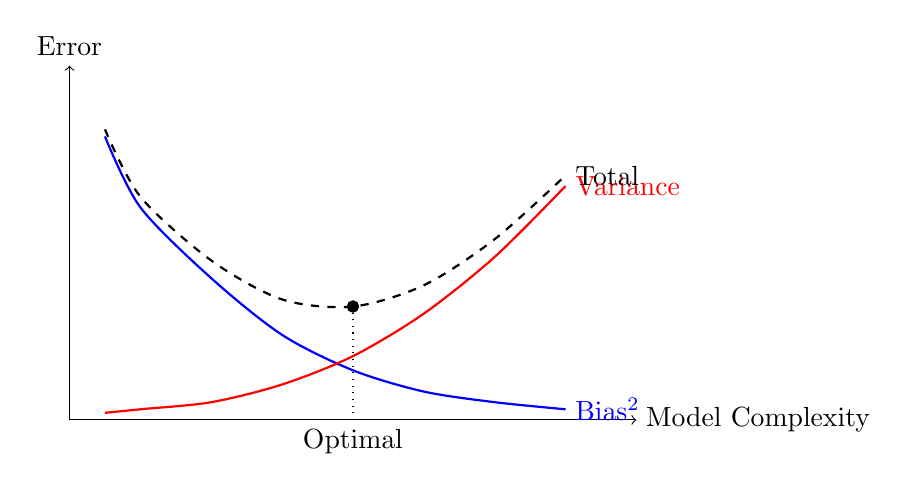
\begin{tikzpicture}[scale=0.9]
    \draw[->] (0,0) -- (8,0) node[right] {Model Complexity};
    \draw[->] (0,0) -- (0,5) node[above] {Error};

    % Bias curve (decreasing)
    \draw[thick, blue] plot[smooth] coordinates {(0.5,4) (1,3) (2,2) (3,1.2) (4,0.7) (5,0.4) (6,0.25) (7,0.15)};
    \node[blue, right] at (7,0.15) {Bias$^2$};

    % Variance curve (increasing)
    \draw[thick, red] plot[smooth] coordinates {(0.5,0.1) (1,0.15) (2,0.25) (3,0.5) (4,0.9) (5,1.5) (6,2.3) (7,3.3)};
    \node[red, right] at (7,3.3) {Variance};

    % Total error (sum)
    \draw[thick, black, dashed] plot[smooth] coordinates {(0.5,4.1) (1,3.15) (2,2.25) (3,1.7) (4,1.6) (5,1.9) (6,2.55) (7,3.45)};
    \node[right] at (7,3.45) {Total};

    % Optimal point
    \draw[dotted] (4,0) -- (4,1.6);
    \node[below] at (4,0) {Optimal};
    \draw[fill=black] (4,1.6) circle (0.08);
\end{tikzpicture}
\caption{The bias-variance tradeoff. Simple models have high bias but low variance; complex models have low bias but high variance. The optimal complexity minimizes total prediction error.}
\label{fig:bias_variance}
\end{figure}

The expected prediction error can be decomposed:
\begin{equation}
\text{Expected Error} = \text{Bias}^2 + \text{Variance} + \text{Irreducible Noise}
\label{eq:bias_variance}
\end{equation}

Cross-validation or information criteria help navigate this tradeoff, selecting models complex enough to capture dynamics but simple enough to generalize.

%=============================================================================
\section{Practical Experiment: Identifying DC Motor Dynamics}
\label{sec:sysid_lab}
%=============================================================================

This laboratory demonstrates system identification principles by treating a DC motor as a ``black box'' whose parameters are unknown. Students will apply input signals, record responses, fit models using least squares, and validate predictions.

\subsection{Learning Objectives}

Upon completion, students will be able to design input signals for system identification, collect and preprocess input-output data, formulate and solve the least squares estimation problem, validate identified models using independent test data, and compare data-driven models to physics-based models.

\subsection{Equipment and Setup}

\begin{table}[htbp]
\centering
\caption{Bill of Materials for System Identification Laboratory}
\label{tab:sysid_bom}
\begin{tabular}{lll}
\toprule
\textbf{Component} & \textbf{Specification} & \textbf{Qty} \\
\midrule
Arduino Uno/Nano & ATmega328P microcontroller & 1 \\
DC Motor with Encoder & 12V, 200+ PPR quadrature encoder & 1 \\
Motor Driver & L298N or TB6612FNG H-bridge & 1 \\
Power Supply & 12V, 2A DC adapter & 1 \\
Computer & MATLAB, Python, or similar & 1 \\
\bottomrule
\end{tabular}
\end{table}

The motor is treated as a ``black box''---we pretend not to know its electrical and mechanical parameters, though for validation we will compare with a physics-based model.

\subsection{System Model}

A DC motor velocity response to armature voltage can be modeled as a first-order system:
\begin{equation}
G(s) = \frac{\omega(s)}{V(s)} = \frac{K}{\tau s + 1}
\label{eq:motor_first_order}
\end{equation}
where $K$ is the DC gain (rad/s per volt) and $\tau$ is the time constant.

In discrete time with sampling period $T_s$:
\begin{equation}
\omega[k] = a_1 \omega[k-1] + b_1 v[k-1] + e[k]
\label{eq:motor_discrete}
\end{equation}

The continuous-time parameters relate to discrete parameters via:
\begin{align}
a_1 &= e^{-T_s/\tau} \\
b_1 &= K(1 - e^{-T_s/\tau}) = K(1 - a_1)
\end{align}

Inverting:
\begin{align}
\tau &= \frac{-T_s}{\ln(a_1)} \label{eq:tau_recovery}\\
K &= \frac{b_1}{1 - a_1} \label{eq:k_recovery}
\end{align}

\subsection{Experimental Procedure}

\subsubsection{Part 1: Data Collection}

\begin{algorithm}
\caption{Data Collection for System Identification}
\label{alg:sysid_data_collection}
\begin{algorithmic}[1]
\State \textbf{Initialize:} Configure motor PWM pins and encoder interrupt pins
\State \textbf{Initialize:} Set sampling period $T_s \gets 0.02$ s (50 Hz)
\State \textbf{Initialize:} Initialize PRBS shift register $\gets 1$
\State \textbf{Initialize:} $\text{encoderCount} \gets 0$, $\text{lastCount} \gets 0$
\State Output CSV header: ``time\_ms, pwm, velocity''
\State Wait 1 second for system stabilization
\While{data collection active}
    \State $\text{currentTime} \gets$ system time in milliseconds
    \If{$\text{currentTime} - \text{lastSampleTime} \geq T_s \times 1000$}
        \State $\text{lastSampleTime} \gets \text{currentTime}$
        \State \Comment{Generate PRBS input signal}
        \State $\text{newBit} \gets (\text{shiftReg}[6] \oplus \text{shiftReg}[5]) \land 1$
        \State $\text{shiftReg} \gets (\text{shiftReg} \ll 1) \lor \text{newBit}$
        \If{$\text{shiftReg} \land 1 = 1$}
            \State $\text{pwmValue} \gets 150$ \Comment{High level}
        \Else
            \State $\text{pwmValue} \gets 80$ \Comment{Low level}
        \EndIf
        \State Apply PWM signal to motor
        \State \Comment{Measure velocity from encoder}
        \State $\text{currentCount} \gets \text{encoderCount}$
        \State $\text{velocity} \gets (\text{currentCount} - \text{lastCount}) / T_s$
        \State $\text{lastCount} \gets \text{currentCount}$
        \State Log: currentTime, pwmValue, velocity
    \EndIf
\EndWhile
\end{algorithmic}
\end{algorithm}

\begin{algorithm}
\caption{Encoder Update (Interrupt Service Routine)}
\label{alg:encoder_update}
\begin{algorithmic}[1]
\State Read encoder channel A and channel B
\If{channel A $=$ channel B}
    \State $\text{encoderCount} \gets \text{encoderCount} + 1$
\Else
    \State $\text{encoderCount} \gets \text{encoderCount} - 1$
\EndIf
\end{algorithmic}
\end{algorithm}

\textbf{Procedure}: Upload the code and connect the motor. Open Serial Monitor and copy data to a file, collecting at least 3000 samples. Split the data, using the first 2000 samples for estimation and the remainder for validation.

\subsubsection{Part 2: Parameter Estimation in MATLAB/Python}

\begin{algorithm}
\caption{Least Squares Parameter Estimation}
\label{alg:sysid_estimation}
\begin{algorithmic}[1]
\State \textbf{Input:} Data file containing time, input $u$, and output $y$ measurements
\State \textbf{Output:} Estimated parameters $\hat{a}_1$, $\hat{b}_1$, $\hat{\tau}$, $\hat{K}$
\State
\State \Comment{Load and partition data}
\State Load data matrix from CSV file
\State $\mathbf{t} \gets$ time column (convert to seconds)
\State $\mathbf{u} \gets$ input column (PWM values)
\State $\mathbf{y} \gets$ output column (velocity)
\State
\State \Comment{Split into estimation and validation sets}
\State $N_{\text{est}} \gets 2000$
\State $\mathbf{u}_{\text{est}} \gets \mathbf{u}[1:N_{\text{est}}]$, \quad $\mathbf{y}_{\text{est}} \gets \mathbf{y}[1:N_{\text{est}}]$
\State $\mathbf{u}_{\text{val}} \gets \mathbf{u}[N_{\text{est}}+1:\text{end}]$, \quad $\mathbf{y}_{\text{val}} \gets \mathbf{y}[N_{\text{est}}+1:\text{end}]$
\State
\State \Comment{Build regression matrix for ARX(1,1): $y[k] = a_1 y[k-1] + b_1 u[k-1] + e[k]$}
\State $\boldsymbol{\Phi} \gets [\mathbf{y}_{\text{est}}[1:N-1], \; \mathbf{u}_{\text{est}}[1:N-1]]$
\State $\mathbf{Y} \gets \mathbf{y}_{\text{est}}[2:N]$
\State
\State \Comment{Solve normal equations}
\State $\hat{\boldsymbol{\theta}} \gets (\boldsymbol{\Phi}^\top \boldsymbol{\Phi})^{-1} \boldsymbol{\Phi}^\top \mathbf{Y}$
\State $\hat{a}_1 \gets \hat{\boldsymbol{\theta}}[1]$, \quad $\hat{b}_1 \gets \hat{\boldsymbol{\theta}}[2]$
\State
\State \Comment{Convert to continuous-time parameters}
\State $\hat{\tau} \gets -T_s / \ln(\hat{a}_1)$
\State $\hat{K} \gets \hat{b}_1 / (1 - \hat{a}_1)$
\State
\State \Comment{Compute parameter uncertainty}
\State $\mathbf{e} \gets \mathbf{Y} - \boldsymbol{\Phi} \hat{\boldsymbol{\theta}}$ \Comment{Residuals}
\State $\hat{\sigma}^2 \gets \text{var}(\mathbf{e})$
\State $\text{Cov}(\hat{\boldsymbol{\theta}}) \gets \hat{\sigma}^2 (\boldsymbol{\Phi}^\top \boldsymbol{\Phi})^{-1}$
\State $\sigma_{a_1} \gets \sqrt{\text{Cov}(\hat{\boldsymbol{\theta}})_{11}}$, \quad $\sigma_{b_1} \gets \sqrt{\text{Cov}(\hat{\boldsymbol{\theta}})_{22}}$
\State
\State \Return $\hat{a}_1$, $\hat{b}_1$, $\hat{\tau}$, $\hat{K}$, $\sigma_{a_1}$, $\sigma_{b_1}$
\end{algorithmic}
\end{algorithm}

\subsubsection{Part 3: Model Validation}

\begin{algorithm}
\caption{Model Validation}
\label{alg:sysid_validation}
\begin{algorithmic}[1]
\State \textbf{Input:} Validation data $\mathbf{u}_{\text{val}}$, $\mathbf{y}_{\text{val}}$; estimated parameters $\hat{a}_1$, $\hat{b}_1$
\State \textbf{Output:} Fit percentage, residual analysis
\State
\State \Comment{Simulate identified model on validation data}
\State Initialize $\hat{\mathbf{y}}_{\text{sim}}$ as zero vector of length $N_{\text{val}}$
\State $\hat{y}_{\text{sim}}[1] \gets y_{\text{val}}[1]$ \Comment{Use measured initial condition}
\For{$k = 2$ \To $N_{\text{val}}$}
    \State $\hat{y}_{\text{sim}}[k] \gets \hat{a}_1 \cdot \hat{y}_{\text{sim}}[k-1] + \hat{b}_1 \cdot u_{\text{val}}[k-1]$
\EndFor
\State
\State \Comment{Compute fit percentage}
\State $\text{FIT} \gets 100 \times \left(1 - \frac{\|\mathbf{y}_{\text{val}} - \hat{\mathbf{y}}_{\text{sim}}\|}{\|\mathbf{y}_{\text{val}} - \bar{y}_{\text{val}}\|}\right)$
\State
\State \Comment{Residual analysis}
\State $\boldsymbol{\varepsilon} \gets \mathbf{y}_{\text{val}} - \hat{\mathbf{y}}_{\text{sim}}$
\State Plot residuals $\boldsymbol{\varepsilon}$ versus time
\State
\State \Comment{Compute autocorrelation of residuals}
\For{$\tau = -50$ \To $50$}
    \State $R_\varepsilon[\tau] \gets$ normalized cross-correlation at lag $\tau$
\EndFor
\State Plot autocorrelation with 95\% confidence bounds $\pm 1.96/\sqrt{N_{\text{val}}}$
\State
\State \Comment{Assess whiteness: residuals are white if ACF within bounds for $\tau \neq 0$}
\State \Return FIT, $\boldsymbol{\varepsilon}$, $R_\varepsilon$
\end{algorithmic}
\end{algorithm}

\subsection{Comparison with Physics-Based Model}

For a DC motor, first-principles analysis yields:
\begin{align}
\tau_\text{physics} &= \frac{JR}{K_t K_e + bR} \label{eq:tau_physics}\\
K_\text{physics} &= \frac{K_t}{K_t K_e + bR} \label{eq:k_physics}
\end{align}
where $J$ is moment of inertia, $R$ is armature resistance, $K_t$ is torque constant, $K_e$ is back-EMF constant, and $b$ is viscous friction.

Students should look up the motor datasheet parameters, calculate $\tau_\text{physics}$ and $K_\text{physics}$, compare these with the identified values $\tau$ and $K$, and discuss sources of discrepancy such as unmodeled friction, driver nonlinearity, and other effects.

\subsection{Data Recording Table}

\begin{table}[htbp]
\centering
\caption{System Identification Results}
\label{tab:sysid_results}
\begin{tabular}{lccc}
\toprule
\textbf{Parameter} & \textbf{Identified} & \textbf{Physics-Based} & \textbf{Difference} \\
\midrule
Time constant $\tau$ (s) & & & \\
DC gain $K$ & & & \\
Validation fit (\%) & & N/A & \\
\bottomrule
\end{tabular}
\end{table}

%=============================================================================
\section{Worked Examples}
\label{sec:sysid_examples}
%=============================================================================

\begin{examplebox}[First-Order System Least Squares Setup]
A first-order system $G(s) = \frac{K}{\tau s + 1}$ is sampled at $T_s = 0.1$ s. Set up the least squares problem to estimate the discrete-time ARX(1,1) parameters.

\textbf{Solution:}

The continuous-time differential equation is:
\begin{equation*}
\tau \dot{y} + y = Ku
\end{equation*}

Discretizing using the forward Euler approximation or exact discretization:
\begin{equation*}
y[k] = e^{-T_s/\tau} y[k-1] + K(1 - e^{-T_s/\tau}) u[k-1]
\end{equation*}

Defining $a_1 = e^{-T_s/\tau}$ and $b_1 = K(1 - e^{-T_s/\tau})$:
\begin{equation*}
y[k] = a_1 y[k-1] + b_1 u[k-1] + e[k]
\end{equation*}

The regression vector is:
\begin{equation*}
\boldsymbol{\phi}[k] = \begin{bmatrix} y[k-1] \\ u[k-1] \end{bmatrix}
\end{equation*}

The parameter vector is:
\begin{equation*}
\boldsymbol{\theta} = \begin{bmatrix} a_1 \\ b_1 \end{bmatrix}
\end{equation*}

For $N$ data points $(k = 2, \ldots, N+1)$:
\begin{equation*}
\boldsymbol{\Phi} = \begin{bmatrix}
y[1] & u[1] \\
y[2] & u[2] \\
\vdots & \vdots \\
y[N] & u[N]
\end{bmatrix}, \quad
\mathbf{y} = \begin{bmatrix}
y[2] \\
y[3] \\
\vdots \\
y[N+1]
\end{bmatrix}
\end{equation*}

The least squares solution is:
\begin{equation*}
\boxed{\hat{\boldsymbol{\theta}} = (\boldsymbol{\Phi}^T \boldsymbol{\Phi})^{-1} \boldsymbol{\Phi}^T \mathbf{y}}
\end{equation*}
\end{examplebox}

\begin{examplebox}[Parameter Estimation from Step Response]
\label{ex:step_estimation}
The following step response data was collected from a first-order system with a step input of magnitude $u = 5$:

\begin{center}
\begin{tabular}{ccccccccc}
\toprule
$t$ (s) & 0 & 0.5 & 1.0 & 1.5 & 2.0 & 2.5 & 3.0 & 3.5 \\
\midrule
$y$ & 0 & 1.57 & 2.53 & 3.12 & 3.49 & 3.72 & 3.86 & 3.95 \\
\bottomrule
\end{tabular}
\end{center}

Estimate the DC gain $K$ and time constant $\tau$.

\textbf{Solution:}

For a first-order step response:
\begin{equation*}
y(t) = Ku(1 - e^{-t/\tau}) = 5K(1 - e^{-t/\tau})
\end{equation*}

\textbf{Method 1: Graphical/Approximate}

The steady-state value appears to be approaching $5K \approx 4.0$, giving $K \approx 0.8$.

At $t = \tau$, the response reaches $63.2\%$ of steady-state: $0.632 \times 4.0 = 2.53$.
From the data, $y(1.0) = 2.53$, so $\tau \approx 1.0$ s.

\textbf{Method 2: Least Squares}

Define $z = 5K - y$, so $z = 5K e^{-t/\tau}$, and $\ln(z) = \ln(5K) - t/\tau$.

This is linear in $\ln(5K)$ and $-1/\tau$. We can estimate $K$ from the final value and then use linear regression on $\ln(z)$ vs. $t$.

Assuming $5K = 4.0$ (estimated final value):
\begin{center}
\begin{tabular}{ccccccccc}
\toprule
$t$ & 0 & 0.5 & 1.0 & 1.5 & 2.0 & 2.5 & 3.0 & 3.5 \\
\midrule
$z = 4 - y$ & 4.0 & 2.43 & 1.47 & 0.88 & 0.51 & 0.28 & 0.14 & 0.05 \\
$\ln(z)$ & 1.39 & 0.89 & 0.39 & -0.13 & -0.67 & -1.27 & -1.97 & -3.00 \\
\bottomrule
\end{tabular}
\end{center}

Linear regression of $\ln(z)$ vs. $t$:
\begin{equation*}
\ln(z) = 1.386 - 1.003 t
\end{equation*}

Therefore:
\begin{align*}
-\frac{1}{\tau} &= -1.003 \quad \Rightarrow \quad \tau = 0.997 \approx 1.0 \text{ s} \\
\ln(5K) &= 1.386 \quad \Rightarrow \quad 5K = 4.0 \quad \Rightarrow \quad K = 0.8
\end{align*}

\begin{equation*}
\boxed{K = 0.8 \text{ (units/input)}, \quad \tau = 1.0 \text{ s}}
\end{equation*}
\end{examplebox}

\begin{example}[Frequency Response Identification]
\label{ex:freq_id}
Sinusoidal tests on a system yield the following frequency response data:

\begin{center}
\begin{tabular}{cccccc}
\toprule
$\omega$ (rad/s) & 0.1 & 0.5 & 1.0 & 2.0 & 5.0 \\
\midrule
$|G(j\omega)|$ & 0.98 & 0.89 & 0.71 & 0.45 & 0.20 \\
$\angle G(j\omega)$ (deg) & $-5.7°$ & $-26.6°$ & $-45°$ & $-63.4°$ & $-78.7°$ \\
\bottomrule
\end{tabular}
\end{center}

Identify a first-order model $G(s) = \frac{K}{\tau s + 1}$.

\textbf{Solution:}

For a first-order system:
\begin{align*}
|G(j\omega)| &= \frac{K}{\sqrt{1 + (\omega\tau)^2}} \\
\angle G(j\omega) &= -\arctan(\omega\tau)
\end{align*}

\textbf{Using phase data:}

At $\omega = 1.0$ rad/s, $\angle G = -45°$, which implies:
\begin{equation*}
\arctan(\omega\tau) = 45° \quad \Rightarrow \quad \omega\tau = 1 \quad \Rightarrow \quad \tau = 1.0 \text{ s}
\end{equation*}

\textbf{Using magnitude data:}

At DC ($\omega \to 0$), $|G| \to K$. From the data, $|G(0.1)| \approx 0.98 \approx K$.

More precisely, at $\omega = 1.0$ rad/s:
\begin{equation*}
|G| = \frac{K}{\sqrt{1 + 1}} = \frac{K}{\sqrt{2}} = 0.71
\end{equation*}
\begin{equation*}
K = 0.71 \times \sqrt{2} = 1.0
\end{equation*}

\textbf{Verification:}

At $\omega = 2.0$ rad/s:
\begin{equation*}
|G| = \frac{1}{\sqrt{1 + 4}} = \frac{1}{\sqrt{5}} = 0.447 \approx 0.45 \quad \checkmark
\end{equation*}

\begin{equation*}
\boxed{G(s) = \frac{1}{s + 1}}
\end{equation*}
\end{example}

\begin{example}[Confidence Intervals on Parameters]
\label{ex:confidence}
An ARX model was identified from $N = 500$ data points, yielding:
\begin{equation*}
\hat{\boldsymbol{\theta}} = \begin{bmatrix} 0.85 \\ 0.12 \end{bmatrix}, \quad
\boldsymbol{\Phi}^T\boldsymbol{\Phi} = \begin{bmatrix} 450 & 25 \\ 25 & 100 \end{bmatrix}, \quad
\hat{\sigma}^2 = 0.04
\end{equation*}

Compute 95\% confidence intervals for the parameters.

\textbf{Solution:}

The parameter covariance matrix is:
\begin{equation*}
\text{Cov}(\hat{\boldsymbol{\theta}}) = \hat{\sigma}^2 (\boldsymbol{\Phi}^T\boldsymbol{\Phi})^{-1}
\end{equation*}

First, compute the inverse:
\begin{equation*}
(\boldsymbol{\Phi}^T\boldsymbol{\Phi})^{-1} = \frac{1}{450 \times 100 - 25^2} \begin{bmatrix} 100 & -25 \\ -25 & 450 \end{bmatrix}
= \frac{1}{44375} \begin{bmatrix} 100 & -25 \\ -25 & 450 \end{bmatrix}
\end{equation*}

\begin{equation*}
= \begin{bmatrix} 0.00225 & -0.000563 \\ -0.000563 & 0.01014 \end{bmatrix}
\end{equation*}

Then:
\begin{equation*}
\text{Cov}(\hat{\boldsymbol{\theta}}) = 0.04 \times \begin{bmatrix} 0.00225 & -0.000563 \\ -0.000563 & 0.01014 \end{bmatrix}
= \begin{bmatrix} 9.0 \times 10^{-5} & -2.25 \times 10^{-5} \\ -2.25 \times 10^{-5} & 4.06 \times 10^{-4} \end{bmatrix}
\end{equation*}

Standard deviations:
\begin{align*}
\sigma_{a_1} &= \sqrt{9.0 \times 10^{-5}} = 0.0095 \\
\sigma_{b_1} &= \sqrt{4.06 \times 10^{-4}} = 0.0201
\end{align*}

For 95\% confidence with large samples (using $z_{0.975} = 1.96$):
\begin{align*}
a_1 &: 0.85 \pm 1.96 \times 0.0095 = 0.85 \pm 0.019 \\
b_1 &: 0.12 \pm 1.96 \times 0.0201 = 0.12 \pm 0.039
\end{align*}

\begin{equation*}
\boxed{a_1 \in [0.831, 0.869], \quad b_1 \in [0.081, 0.159] \text{ (95\% confidence)}}
\end{equation*}
\end{example}

\begin{example}[Model Validation with Test Data]
\label{ex:validation}
A model identified from training data predicts the following on a validation set of 100 points:

\begin{center}
\begin{tabular}{cc}
\toprule
Quantity & Value \\
\midrule
$\sum_{k=1}^{100} y^2_\text{val}[k]$ & 5000 \\
$\sum_{k=1}^{100} (y_\text{val}[k] - \hat{y}[k])^2$ & 200 \\
Mean of $y_\text{val}$ & 6.5 \\
\bottomrule
\end{tabular}
\end{center}

Compute the fit percentage and NRMSE.

\textbf{Solution:}

\textbf{NRMSE (Normalized Root Mean Square Error):}
\begin{equation*}
\text{NRMSE} = \sqrt{\frac{\sum(y - \hat{y})^2}{\sum y^2}} = \sqrt{\frac{200}{5000}} = \sqrt{0.04} = 0.2 = 20\%
\end{equation*}

\textbf{Fit Percentage:}

First compute $\|y_\text{val} - \bar{y}\|^2$:
\begin{equation*}
\sum_{k=1}^{100} (y_\text{val}[k] - \bar{y})^2 = \sum y^2 - N\bar{y}^2 = 5000 - 100 \times 6.5^2 = 5000 - 4225 = 775
\end{equation*}

Then:
\begin{equation*}
\text{FIT} = 100 \times \left(1 - \frac{\|y - \hat{y}\|}{\|y - \bar{y}\|}\right) = 100 \times \left(1 - \frac{\sqrt{200}}{\sqrt{775}}\right)
\end{equation*}
\begin{equation*}
= 100 \times \left(1 - \frac{14.14}{27.84}\right) = 100 \times (1 - 0.508) = 49.2\%
\end{equation*}

\begin{equation*}
\boxed{\text{NRMSE} = 20\%, \quad \text{FIT} = 49.2\%}
\end{equation*}

A fit of 49\% is marginal---the model captures about half the variance beyond the mean. This suggests the model structure may be inadequate (e.g., first-order for a higher-order system) or there is significant noise.
\end{example}

\begin{example}[Second-Order System Identification]
\label{ex:second_order}
Step response data from a system shows oscillatory behavior with the following characteristics: a final value of $y_{ss} = 2.0$ for step input $u = 1$, a peak value of $y_{peak} = 2.5$ at $t_p = 0.5$ s, and a second peak of $y_{peak2} = 2.1$ at $t = 1.5$ s.

Identify a second-order model $G(s) = \frac{K\omega_n^2}{s^2 + 2\zeta\omega_n s + \omega_n^2}$.

\textbf{Solution:}

\textbf{DC Gain:}
\begin{equation*}
K = \frac{y_{ss}}{u} = \frac{2.0}{1} = 2.0
\end{equation*}

\textbf{Percent Overshoot:}
\begin{equation*}
\%OS = \frac{y_{peak} - y_{ss}}{y_{ss}} \times 100 = \frac{2.5 - 2.0}{2.0} \times 100 = 25\%
\end{equation*}

\textbf{Damping Ratio:}
\begin{equation*}
\%OS = 100 \times e^{-\pi\zeta/\sqrt{1-\zeta^2}}
\end{equation*}
\begin{equation*}
0.25 = e^{-\pi\zeta/\sqrt{1-\zeta^2}}
\end{equation*}
\begin{equation*}
\ln(0.25) = \frac{-\pi\zeta}{\sqrt{1-\zeta^2}}
\end{equation*}
\begin{equation*}
-1.386 = \frac{-\pi\zeta}{\sqrt{1-\zeta^2}}
\end{equation*}

Squaring both sides:
\begin{equation*}
1.922 = \frac{\pi^2\zeta^2}{1-\zeta^2}
\end{equation*}
\begin{equation*}
1.922(1-\zeta^2) = \pi^2\zeta^2
\end{equation*}
\begin{equation*}
\zeta^2 = \frac{1.922}{1.922 + \pi^2} = \frac{1.922}{11.79} = 0.163
\end{equation*}
\begin{equation*}
\zeta = 0.404
\end{equation*}

\textbf{Natural Frequency:}

The peak time is:
\begin{equation*}
t_p = \frac{\pi}{\omega_n\sqrt{1-\zeta^2}} = \frac{\pi}{\omega_d}
\end{equation*}
\begin{equation*}
\omega_d = \frac{\pi}{t_p} = \frac{\pi}{0.5} = 6.28 \text{ rad/s}
\end{equation*}
\begin{equation*}
\omega_n = \frac{\omega_d}{\sqrt{1-\zeta^2}} = \frac{6.28}{\sqrt{1-0.163}} = \frac{6.28}{0.915} = 6.87 \text{ rad/s}
\end{equation*}

\textbf{Final Model:}
\begin{equation*}
\boxed{G(s) = \frac{2 \times 47.2}{s^2 + 5.55s + 47.2} = \frac{94.4}{s^2 + 5.55s + 47.2}}
\end{equation*}
where $\omega_n^2 = 47.2$, $2\zeta\omega_n = 5.55$.
\end{example}

%=============================================================================
\section{System Identification Flowchart}
\label{sec:sysid_flowchart}
%=============================================================================

\begin{figure}[htbp]
\centering
\begin{tikzpicture}[node distance=1.5cm,
    block/.style={rectangle, draw, text width=5cm, text centered, minimum height=1cm, fill=blue!10},
    decision/.style={diamond, draw, text width=3cm, text centered, aspect=2, fill=yellow!20},
    arrow/.style={->, >=stealth, thick}]

% Nodes
\node[block] (design) {1. Design Experiment\\Choose input signal (PRBS, chirp, step)};
\node[block, below=of design] (collect) {2. Collect Data\\Apply input, record output};
\node[block, below=of collect] (preprocess) {3. Preprocess Data\\Remove mean, filter, check quality};
\node[block, below=of preprocess] (select) {4. Select Model Structure\\ARX$(n_a, n_b)$, OE, etc.};
\node[block, below=of select] (estimate) {5. Estimate Parameters\\Least squares, ML, PEM};
\node[decision, below=of estimate] (validate) {6. Validate Model\\Residuals white? Good fit on test data?};
\node[block, below left=1.5cm and -1cm of validate] (increase) {Increase model order};
\node[block, below right=1.5cm and -1cm of validate] (accept) {Accept Model};

% Arrows
\draw[arrow] (design) -- (collect);
\draw[arrow] (collect) -- (preprocess);
\draw[arrow] (preprocess) -- (select);
\draw[arrow] (select) -- (estimate);
\draw[arrow] (estimate) -- (validate);
\draw[arrow] (validate) -- node[left] {No} (increase);
\draw[arrow] (increase) -- ++(-2,0) |- (select);
\draw[arrow] (validate) -- node[right] {Yes} (accept);

\end{tikzpicture}
\caption{System identification workflow. The iterative loop between model structure selection and validation continues until an adequate model is found.}
\label{fig:sysid_flowchart}
\end{figure}

%=============================================================================
\section{Chapter Summary}
\label{sec:sysid_summary}
%=============================================================================

This chapter developed the theory and practice of system identification across several key areas.

\textbf{Historical Foundation}: System identification originated with Gauss's least squares method for orbital prediction (1809) and matured through Ljung's prediction error framework (1970s--80s). The guiding philosophy is ``all models are wrong, some are useful'' (Box).

\textbf{Input Design}: Effective identification requires persistently exciting inputs. PRBS signals provide broadband excitation with bounded amplitude; chirps enable frequency-by-frequency characterization.

\textbf{Least Squares Estimation}: The regression form $\mathbf{y} = \boldsymbol{\Phi}\boldsymbol{\theta} + \mathbf{e}$ leads to the normal equations $\hat{\boldsymbol{\theta}} = (\boldsymbol{\Phi}^T\boldsymbol{\Phi})^{-1}\boldsymbol{\Phi}^T\mathbf{y}$. Under Gaussian noise, this is the Best Linear Unbiased Estimator.

\textbf{ARX Models}: The AutoRegressive with eXogenous input structure $y[k] = a_1 y[k-1] + \cdots + b_1 u[k-1] + \cdots + e[k]$ enables direct least squares estimation. Continuous-time parameters are recovered through conversion formulas.

\textbf{Frequency Domain Methods}: Sinusoidal testing or spectral analysis yields empirical Bode plots. Parametric models can be fitted to frequency data.

\textbf{Model Validation}: Residual whiteness tests and cross-validation on held-out data assess model adequacy. The bias-variance tradeoff governs model complexity selection.

\begin{tcolorbox}[colback=yellow!10!white,colframe=orange!75!black,title=Key Takeaway,sharp corners]
System identification bridges the gap between theoretical models and physical reality. When first-principles modeling is expensive or inaccurate, data-driven identification provides an alternative path to useful models. The key insight: design experiments to maximize information content, fit models using principled estimation methods, and rigorously validate before deployment.
\end{tcolorbox}

%=============================================================================
\newpage
\section{Exercises}
\label{sec:sysid_exercises}
%=============================================================================

\begin{exercise}
\textbf{Regression Form}: Write the ARX(2,2) model
\begin{equation*}
y[k] + a_1 y[k-1] + a_2 y[k-2] = b_1 u[k-1] + b_2 u[k-2] + e[k]
\end{equation*}
in regression form $y[k] = \boldsymbol{\phi}^T[k]\boldsymbol{\theta} + e[k]$. Define $\boldsymbol{\phi}[k]$ and $\boldsymbol{\theta}$.
\end{exercise}

\begin{exercise}
\textbf{Least Squares Derivation}: Derive the normal equations by completing the square on the cost function $J(\boldsymbol{\theta}) = \|\mathbf{y} - \boldsymbol{\Phi}\boldsymbol{\theta}\|^2$.
\end{exercise}

\begin{exercise}
\textbf{Step Response Identification}: The following step response data ($u = 2$) was recorded:
\begin{center}
\begin{tabular}{cccccccc}
\toprule
$t$ (s) & 0 & 1 & 2 & 3 & 4 & 5 & 6 \\
\midrule
$y$ & 0 & 3.16 & 5.07 & 6.22 & 6.93 & 7.36 & 7.62 \\
\bottomrule
\end{tabular}
\end{center}
Estimate $K$ and $\tau$ for a first-order model.
\end{exercise}

\begin{exercise}
\textbf{Frequency Domain Fitting}: Given frequency response measurements $|G(j\omega)| = [0.95, 0.7, 0.45, 0.3]$ at $\omega = [0.5, 1, 2, 3]$ rad/s, fit a first-order model using least squares on $|G|^{-2}$.
\end{exercise}

\begin{exercise}
\textbf{Covariance Analysis}: If $\boldsymbol{\Phi}^T\boldsymbol{\Phi} = \begin{bmatrix} 1000 & 0 \\ 0 & 500 \end{bmatrix}$ and $\sigma^2 = 0.01$, compute the parameter standard deviations. How does doubling the data length (approximately doubling $\boldsymbol{\Phi}^T\boldsymbol{\Phi}$) affect these?
\end{exercise}

\begin{exercise}
\textbf{Model Order Selection}: An engineer identifies ARX models of orders 1 through 5. The validation fit percentages are 65\%, 78\%, 82\%, 83\%, 82\%. Which order should be selected and why?
\end{exercise}

\begin{exercise}
\textbf{PRBS Design}: Design a 7-bit PRBS with clock period 0.1 s. What is its period? What is its approximate bandwidth?
\end{exercise}

\begin{exercise}
\textbf{Laboratory Extension}: Modify the Arduino code to use a chirp input instead of PRBS. Compute the empirical frequency response using FFT in MATLAB/Python.
\end{exercise}

\begin{exercise}
\textbf{Bias Analysis}: An ARX model is fitted to data from a system where the noise is actually filtered (colored). Will the least squares estimate be biased? Explain why.
\end{exercise}

\begin{exercise}
\textbf{Physics Comparison}: A motor has datasheet parameters $R = 5\,\Omega$, $L = 10\,$mH (negligible), $K_t = K_e = 0.05\,$Nm/A, $J = 10^{-4}\,$kg$\cdot$m$^2$, $b = 10^{-5}\,$Nm$\cdot$s/rad. Calculate the theoretical time constant and DC gain. Compare with typical identified values and discuss sources of discrepancy.
\end{exercise}

%=============================================================================
% End of Chapter
%=============================================================================
